\section{Machine Learning and Predictive Modeling}
Machine learning enables computers to perform tasks without manually codifying all instructions.
This automated programming makes machine learning a popular and widely used approach for many applications as it provides a time- and cost-effective alternative to manually created software solutions.
Machine learning relies on algorithms that learn and generalize from examples in order to perform accurately on new or unseen data.

Predictive modeling is a subcategory of machine learning that aims to predict certain properties from given input data.
The input data typically consists of \emph{instances} with a given set of \emph{features}.
The values of those features can be binary, categorical, or numerical.
We can think of the data as a table where features are columns and rows are instances.
Thus, this kind of data is typically referred to as \emph{tabular} or \emph{structured} data.
In the case of \emph{unstructured} data, such as plain text, the data needs to be converted into structured data first, before it can be used as input of predictive models\footnote{In this case, the model input corresponds to a fixed-length transformed representation of the original input data. These transformations can be either learned (\ie, via deep learning or similar methods) or are manually specified.}.
The predicted property, \emph{outcome} or \emph{label}, can be numerical, in which case the task is called \emph{regression}, or categorical, in which case the task is called \emph{classification}\footnote{A combination of multiple properties are also possible to predict, in which case the task is called multitask learning, structured learning, \etc. Currently, the most common form of predictive modeling involves either a single classification or single regression task.}.
The different values the label can assume are called \emph{classes}.
The task is call \emph{binary classification} if the categorical label has exactly two classes.

The predictive model learns by \emph{training} with a set of example instances (\emph{training set}) and their associated labels.
In order to verify that the model did indeed correctly learn from the given examples, a second, previously unseen, set of example instances (testing or \emph{validation set}) with known labels is typically used.
The model is used to predict the labels of this set which are then compared to the actual labels of those instances.
Various statistical measures can be computed on this relationship between the predicted and actual labels \cite{mlbook}.

For binary classification tasks (for simplicity \emph{positive} and \emph{negative} are used below to describe the outcomes) those statistical measures include:

\begin{description}[noitemsep]
    \item[True Positive / Negative]
    The number of correctly predicted positive ($TP$) or negative instances ($TN$).
    \item[False Positive / Negative]
    The number of incorrectly predicted positive ($FP$) or negative instances ($FN$).
    \item[Accuracy]
    $(TP + TN) / (TP + TN + FP + FN)$ The proportion of correctly predicted instances.
    \item[Precision]
    $TP / (TP + FP)$ The ratio of correctly predicted positive instances to instances which were predicted to be positive.
    \item[True Positive Rate / Recall]
    $TP / (TP + FN)$ The proportion of correctly predicted positive instances.
    \item[False Positive Rate]
    $FP / (FP + TN)$ The proportion of incorrectly predicted positive instances.
\end{description}

Additionally, a further model quality measurement can be derived from the confidence of a model in its prediction.
Typically, classification models allow to output probabilities for each class instead of the predicted class directly.
This allows for inspecting the \emph{confidence} of the model.
In the case of binary classifiers a \emph{threshold} can be used to adjust predictions to favor confidence in a certain class higher than the other.
This is achieved by outputting the positive class as prediction if its probability is higher than the threshold and the negative class otherwise.

\begin{figure}
\centering
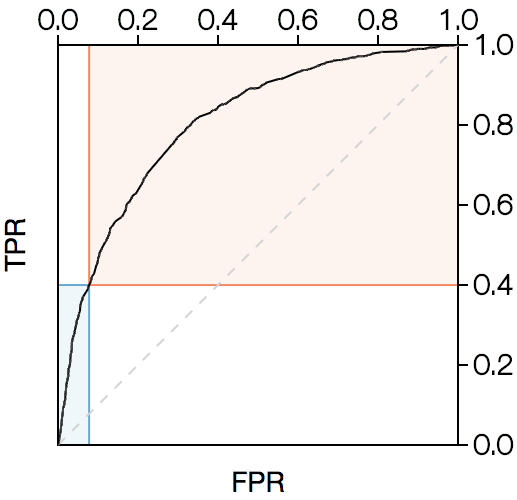
\includegraphics[height=10em]{figs/roc}
\caption[Example of a ROC curve.]{
Example of a ROC curve. The threshold minimizing incorrect predictions is highlighted by the colored axes.
}
\label{figs:roc_intro}
\end{figure}

The \emph{receiver operating characteristic} (ROC) curve for binary classifiers plots the true positive rate against the false positive rate for all thresholds between $0$ and $1$.
The plot indicates the correctness of the model \wrt its confidence.
The ROC curve for a perfect model ($100\%$ accuracy) would follow the left vertical axis and the top horizontal axis.
The area under the ROC curve (\emph{AUC}) is a commonly used measure for model quality \cite{bradley19971145}.

\subsection{Popular Algorithms}
There are too many algorithms for predictive models to list all of them here.
However, following we will discuss the most commonly used algorithms.

\subsubsection{Logistic Regression}
Logistic Regression \cite{mlbook} is one of the most popular algorithms in machine learning.
This is due to its simplicity and its interpretability of the results.
Suppose $x_i$ is the value of the feature $i$ of our data, a binary classification using Logistic Regression is equivalent to:
\[
l(x) = b + \sum_{i \in \mathcal{C}} w_i x_i
\]
where $\mathcal{C}$ is the set of features, $b$ and $w_i$ are the learned weights of the model, and the outcome is determined by whether the weighted sum $l(x)$ is larger or smaller than zero.
In order to work with probabilities, have greater precision around the boundary, and to penalize points close to the boundary, a logistic function is used:
\[
P(Y=1 | x) = L(x) = \frac{1}{1 + e^{-l(x)}}
\]
which gives the likelihood of one of the classes.
In order to train the model, \ie, finding the best values of $b$ and $w_f$, the expression $P(Y=y | x)$, where $y$ represents the ground truth 0 or 1 of the training instances, needs to be maximized.
In practice, instead of maximizing $P(Y=y|x)$, the negative logarithm of this expression is minimized.
When optimized over the entire training data, this expression is called \emph{negative log likelihood} and it can be optimized via techniques such as gradient descent, to find optimal values of $b$ and $w_f$.

One of the main advantages of logistic regression is its interpretability.
The weights $w_i$ can be directly interpreted as how influential a particular feature is.
That is, if the magnitude of a weight is large, a small change in the value $x_i$ of the feature has a big impact on the overall sum.
Additionally, the sign of a weight indicates whether a particular feature is positively or negatively correlated with the outcome.
For example, a simple (not necessarily correct) predictor for Type 2 Diabetes\footnote{A disease, affecting the body's ability to regulate blood sugar, which is mostly driven by lifestyle choices and associated with obesity and hypertension. The most common age of onset is between ${\sim}45$ and ${\sim}65$.} could look like:
\[
l_\text{diabetes}(x) = -1.9 + 0.01 x_\text{age} + 0.02 x_\text{mass} + (-0.3) x_\text{height}
\]
with $x_\text{age}$ in years, $x_\text{mass}$ in \si{kg}, and $x_\text{height}$ in \si{m}.
From here, we can see that the model assumes that a high mass leads to higher Diabetes risk, old age also leads to a higher risk but less so than high mass, and large body height leads to a smaller risk.
This gives a very intuitive understanding of how the model is reaching its conclusion.

However, this example also illustrates some limitations of logistic regression models.
BMI (Body Mass Index; $x_\text{mass} / x_\text{height}^2$) is a better indicator than mass or height alone, but cannot be expressed or learned by a logistic regression model\footnote{Note, that we could provide BMI directly but only because domain experts had inferred the importance of this relationship in the past. Alternatively, we could also provide features in logarithmic space enabling logistic regression models to learn this relationship, since logarithmic BMI is $\log{(x_\text{mass})} - 2.0 \log{(x_\text{height})}$.}.
Additionally, since the influence of the features is always the same, one feature can force a prediction if its values are large enough.
For example, the model will predict a high Diabetes risk with high age independent of the mass or height.

\subsubsection{Generalized Additive Models}
A Generalized Additive Model (GAM \cite{gam}) extends the idea of logistic regression to functions instead of weights:
\[
g(x) = b + \sum_{i \in \mathcal{C}} f_i(x_i)
\]
where $\mathcal{C}$ is the set of features, $b$ is the learned bias of the model, $f_i$ are learned influence functions, and the outcome is determined by whether the sum $g(x)$ is larger or smaller than zero.
Having influence functions overcomes the restricted expressiveness of logistic regression models while maintaining its interpretability.
The impact of individual features can be seen in the plots of the influence functions.

\begin{figure}
\centering
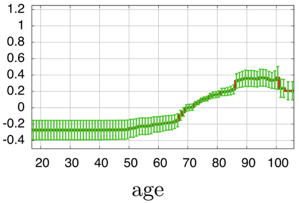
\includegraphics[height=8em,valign=t]{tex/introduction/age.png}
\caption[Influence function for ``age" from a Generalized Additive Model.]{
An influence function for ``age" from a Generalized Additive Model \cite{Caruana:2015:IMH:2783258.2788613}.
}
\label{figs:age}
\end{figure}

In the Diabetes example from above, a GAM could solve the issue of always connecting high age to high Diabetes risk by decreasing the influence of the feature age for higher values than ${\sim}65$.
However, since GAMs only consider one feature at a time, the BMI ($x_\text{mass} / x_\text{height}^2$) can still not be expressed or learned by the model.

\subsubsection{Decision Trees}
Instead of computing predictions with a mathematical formula, Decision Trees \cite{mlbook} determine predictions by following a sequence of tests on the data.
Decision Trees are trees where each node represents a test $x_i > t_i$, with $x_i$ as the value of the feature $i$ and $t_i$ as learned threshold.
The prediction algorithm starts at the root of the tree.
Depending on the outcome of the test in the root node the algorithm continues with the corresponding sub-tree recursively, until a leaf node is reached.
The leaf nodes contain the probabilities for the outcomes of the prediction task and are returned as result by the algorithm.

\begin{figure}
    \centering
    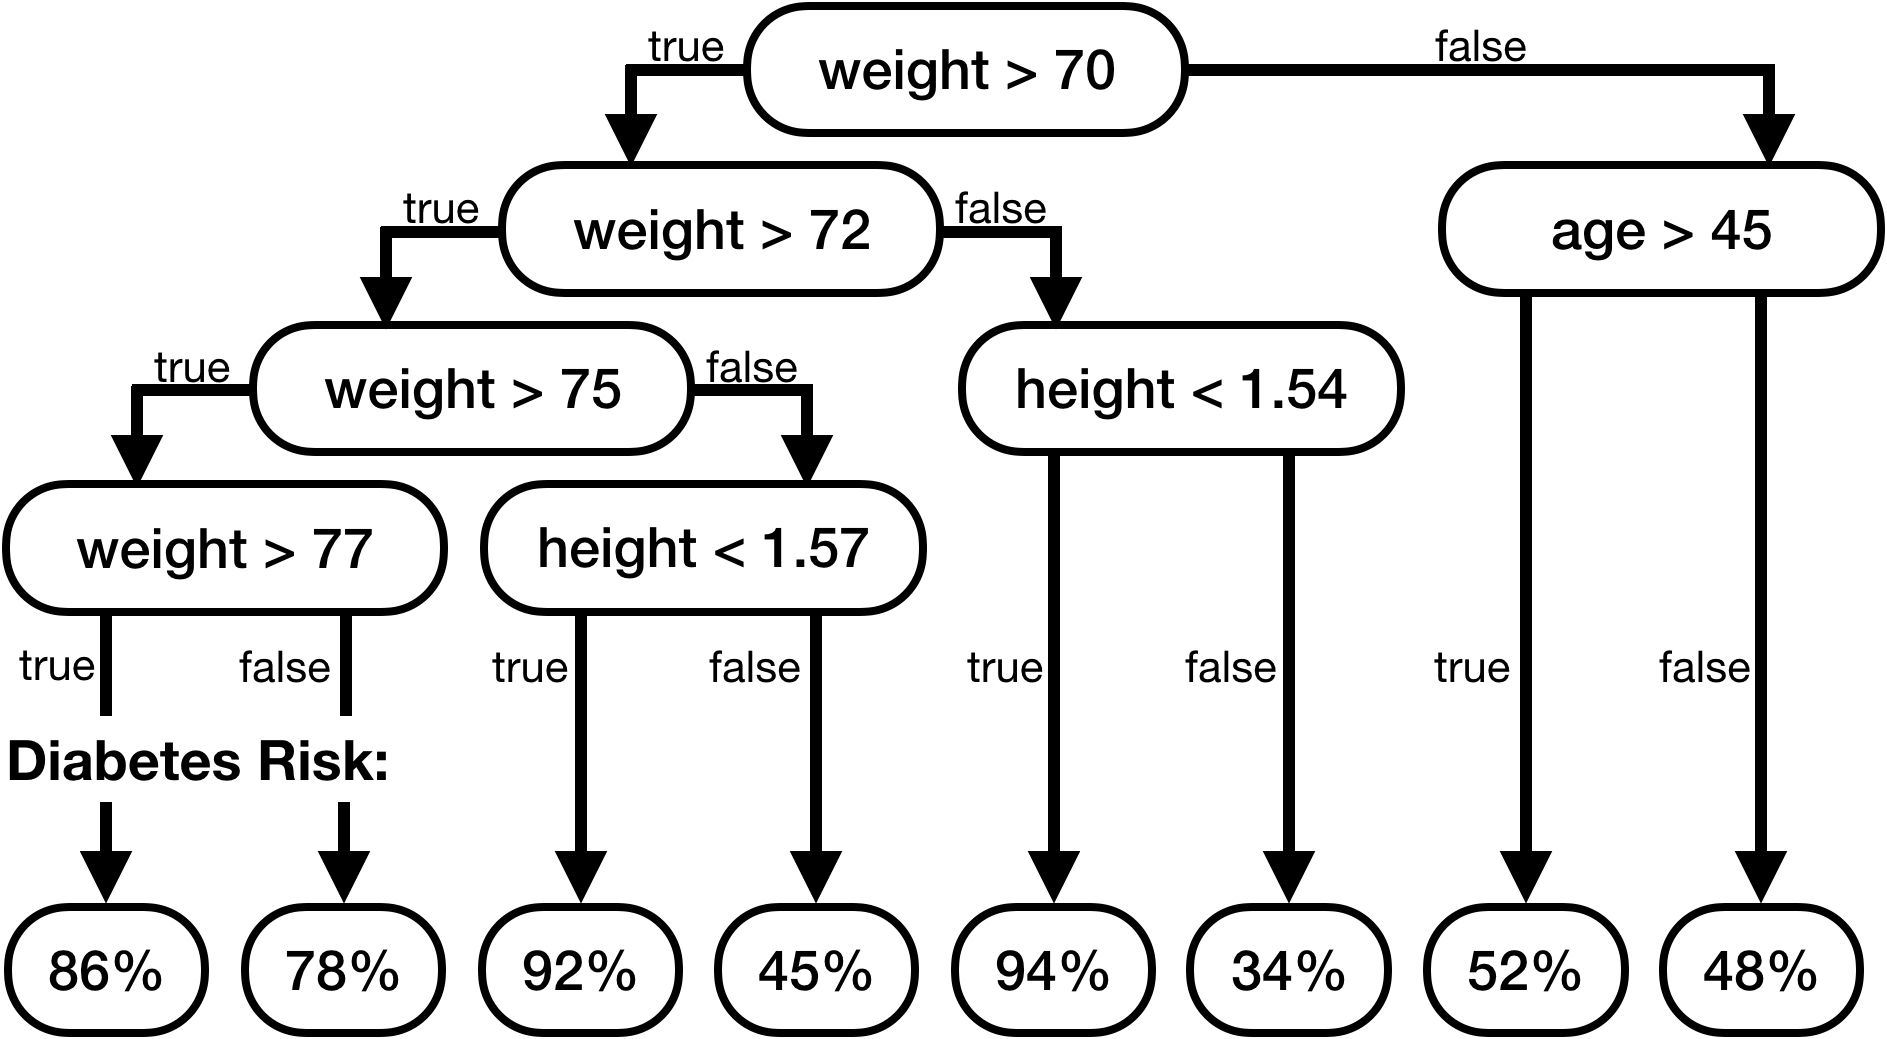
\includegraphics[width=0.9\linewidth]{tex/decisiontree}
    \caption[Example Decision Tree]{A possible decision tree for the Diabetes prediction example\footnotemark. Note, that the tree has interval checks to model the relationship between ``weight'' in \si{kg} and ``height'' in \si{m}.}
    \label{figs:dctree}
\end{figure}
\footnotetext{The decision tree or its parameters are \emph{not} based on data and serve only illustratory purposes.}

Decision Trees are usually considered very interpretable, as their behaviour is intuitively understandable.
However, this only holds true for trees with a relatively low number of nodes.
Trees with hundreds or thousands of nodes are hard to interpret as their complexity makes it hard to gain a mental model.

Decision Trees excel in cases where certain ranges of features have a clear impact on the outcome.
For example, in our running Diabetes use case, the risk of becoming diabetic is significantly higher for ages between ${\sim}45$ and ${\sim}65$.
A Decision Tree can then differentiate by age and infer the prediction differently for values inside or outside of that range.

However, Decision Trees cannot model relationships between features very well and have to approximate them.
For example, increasing the height of a person also increases that person's weight.
This means that whether a person is overweight, not only depends on the weight of the person, but also how tall that person is.
A person weighing $80\si{kg}$ can be considered overweight with a height of $1.7\si{m}$ but would not be with a height of $1.8\si{m}$.
Since a Decision Tree cannot model this relationship ($x_\text{mass} / x_\text{height}^2 \geq 25$) directly it has to approximate it by breaking the values of $x_\text{mass}$ and $x_\text{height}$ into intervals and checking them separately (see Figure~\ref{figs:dctree}).
Because of this, Decision Trees are likely to over-fit on the training data.
Over-fitting happens when a machine learning model does not generalize well because of a pattern in the data that is only present in the training data.

\subsubsection{Ensemble Methods}
A powerful method of utilizing several weak models are Ensemble Models.
Instead of taking the prediction of one model, Ensembles combine the prediction of many models in order to get a definite result.
This is typically done either by using the average prediction of multiple models or by majority voting, \ie, the most common prediction among the individual models is used as final prediction \cite{mlbook}.

The main advantage of Ensemble Models is that it can improve the performance of otherwise worse performing models.
Given a set of independent / uncorrelated models the error reduction of the Ensemble is proportional to the number of individual models \cite{dlbook}. % chapter 7.11

One popular Ensemble Model is the Random Forest~\cite{Breiman:2001:RF:570181.570182}, which combines several Decision Trees trained on random sub-samples of the training data.
This overcomes the tendency of Decision Trees to over-fit on their training data.
Another advantage of Random Forests is that they typically produce good results on only few training instances already.

\subsubsection{Neural Networks}
With the recent advance of more powerful computation hardware, especially with highly parallelizable GPUs\footnote{Graphics Processing Unit}, and availability of larger data sets, (Deep) Neural Networks have become a popular class of machine learning models.
The basic building block of a Neural Network is a \emph{layer}, that is a mathematical construct that has $N$ input features and $M$ output features.
A layer can also have stored coefficients called \emph{weights}.

A very common layer is the fully-connected layer.
For each output feature or \emph{node}, it computes a weighted sum of all input features, much like Linear Regression:
\[
y_j(x) = b_j + \sum^{N}_{i = 1} w_{ij} x_i
\]
where the $y_j$ represents the $j$th output feature, $b_j$ is the corresponding bias and $w_{ij}$ the corresponding weights.

Other common layers are ReLU (Rectified Linear Unit) and Softmax which both require $N = M$.
ReLU computes as $y_j(x) = \max{(0, x_j)}$ which basically acts as filter to let only positive values through.
Softmax computes as $y_j(x) = e^{x_j} / \sum^{N}_{i = 1} e^{x_i}$ and scales the input vector in a way that the output vector sums to one.

With those layers we can build a Multi-Layer-Perceptron (MLP \cite{mlp}) classifier.
A MLP chains a number of fully-connected layers and ReLUs (or other non-linear functions) to each other.
This can be interpreted as a sequence of 1. transform the input, 2. filter out negative values, 3. repeat.
Softmax is used as final layer to compute the actual classification.
Each node here represents one of the classes of the classifier and the class with the highest value ``wins".

Training a MLP or any Neural Network works as follows.
We initialize all weights with random numbers.
%\footnote{Other initialization methods such as Xavier also exist.}
For each instance of the training data set, we first compute the outcome with the current weights.
Then we compute the gradient of the loss function, (which can be either the negative log likelihood of training data labels for classification or mean of squared error for regression tasks), with respect to each parameter.
The gradient is computed on the predicted outcome $y(x)$ (\ie, values of the final layer) and the \emph{desired} outcome $\hat{y}(x)$ (\ie, value of desired class set to one and zero otherwise).
Then, going in reverse order we numerically compute this gradient for each layer and nudge the weights of those layers into the direction of the gradient.
This procedure is called back-propagation.
Ideally, we repeat back-propagation until all weights converge towards fixed numbers, at which point the model is trained.

Neural networks are a powerful machine learning tool, as they enable any function to be modeled \cite{hornik1991251} and allow for great flexibility through combining different layers.
Multi-Layer Perceptrons can potentially be used on our running Diabetes example from above, as they do not have the limitations of any of the previously discussed models.
However, neural networks typically require many thousand training examples in order to properly converge towards a performant model, making them a sub-optimal choice for tasks where acquiring data is time-consuming or expensive.

\subsection{Failure Modes}
Machine learning models not always perform perfectly.
In general, for a given data set, failures to do so typically fall into two main categories: under- and over-fitting \cite{mlbook}.

Under-fitting occurs when a model does not have enough \emph{capacity} to fully learn the input data.
For example, a Logistic Regression model will never be able to learn to classify whether a point lies inside or outside of a circle, using Cartesian coordinates as input features.
This is due to the linear nature of the model.
Under-fitting can be prevented by using a more powerful model or increasing the capacity of the current model.

Over-fitting occurs when a model learns its training data set too precisely.
For example, a Decision Tree might create one leaf node for every instance in the training data memorizing the outcomes of the training data in full.
In this case the model likely won't generalize to new, unseen data.
Thus, in order to detect over-fitting, it is common to keep a separate data set, called hold-out or test data set, at hand that is not used for training the model.
The trained model is then tested against this data set.
If the model performs well on the training data but not on the test data, then it is over-fitting.
A way to prevent this is to reduce the capacity of the model.
For example, reducing the allowed maximum depth of a Decision Tree model is a good way to reduce its capacity.

However, not all failures of machine learning models can be ascribed to the quality of the model.
Failures can also stem from the quality of the data.
Common cases include:

\par \noindent \textbf{Biased Data:}
Biased data might occur if the acquired data stems from a sub-population that insufficiently represents the entire population.
For example, if we train our Diabetes model from above only with obese people the resulting model will most likely have a greater tendency to predict Diabetes.

\par \noindent \textbf{Leaking Labels:}
If a feature of the data is highly correlated to the outcome, a model might only learn this connection, preventing the model to generalize properly.
For example, including an additional feature ``Takes Insulin" to the Diabetes model would leak the label, as only people that are already diagnosed with Type 2 Diabetes take the drug Insulin.

\section{Visual Analytics}
Gaining meaningful insights about large data sets is hard.
While computing various statistics about the data is often helpful it might oversimplify or in some cases even mislead information about the data.
One example data set often used to demonstrate this is Anscombe's quartet~\cite{doi:10.1080/00031305.1973.10478966}.
The quartet consists of four different data sets that all have the same mean and sample variance for both axes, the same correlation between the axes, and the same regression lines.
However, plotting the values of the data sets reveals that each one of those data sets obeys a different, unique characteristic (see Figure~\ref{figs:anscombe}).

\begin{figure*}[t]
\centering
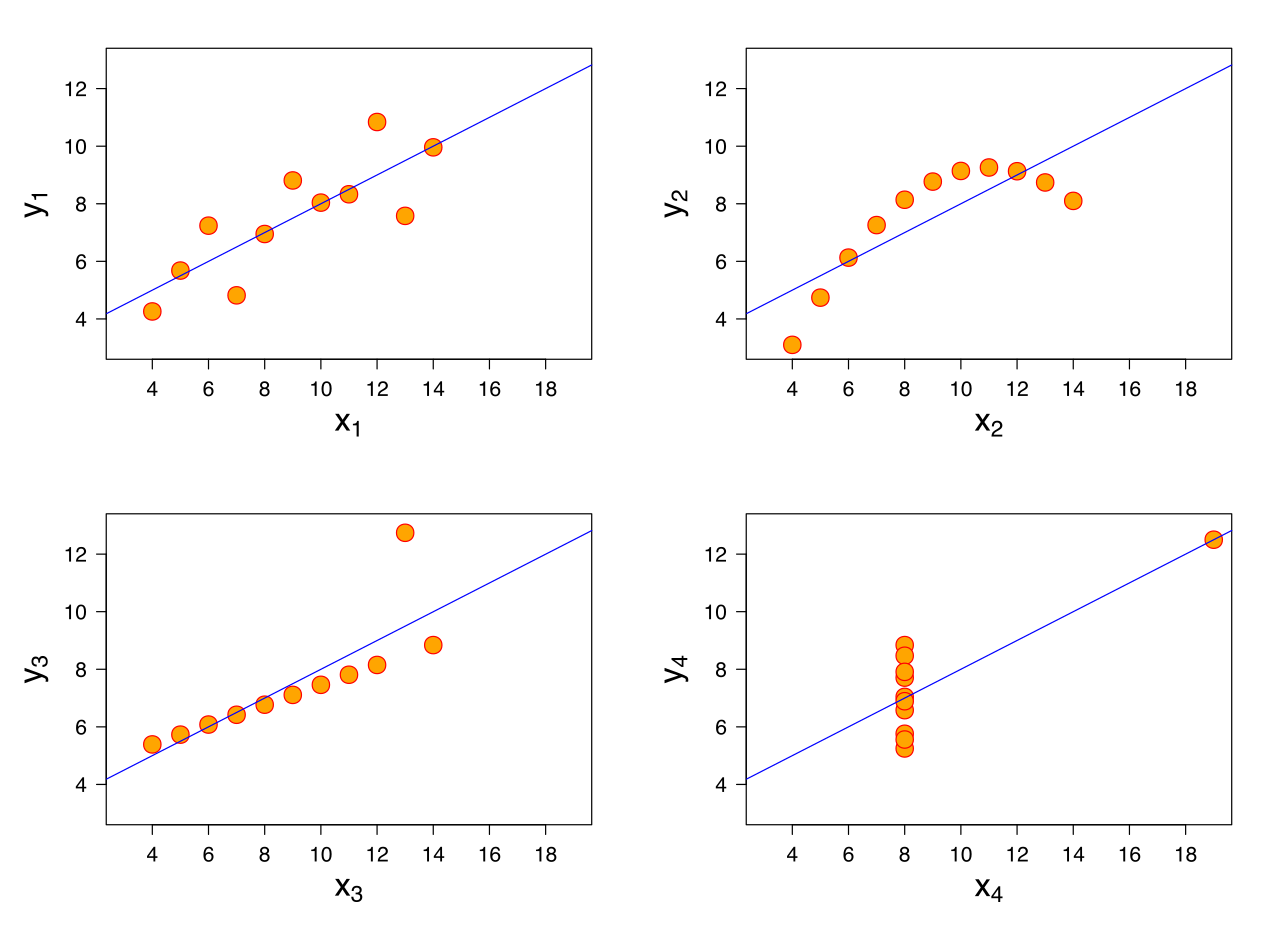
\includegraphics[width=0.9\textwidth,valign=t]{tex/introduction/anscombe.png}
\caption[Anscombe's quartet.]{
Plots of the four data sets of Anscombe's quartet\footnotemark. All data sets have the same mean and sample variance for both axes, the same correlation between the axes, and the same regression lines.
}
\label{figs:anscombe}
\end{figure*}
\footnotetext{Image source: Wikipedia}

Visual Analytics is the area of studying interactive graphical respresentations for analyzing complex data such as Anscombe's quartet mentioned above.
This is often done in addition to and with the help of computational and statistical procedures.
Various studies \cite{doi:10.1080/01621459.1984.10478080,Treisman:1985:PPV:5088.5091,Chang:2002:GTV:820060.820062} have been performed to establish visual principles to effectively take advantage of the high processing power of the human visual system.
Additionally, interaction with the graphical representations allows to hide some of the information and reveal it through interaction to not overwhelm the analyst.
For example, ``overview first; details on demand"~\cite{Shneiderman96theeyes} is a popular mantra taking advantage of interaction.

In the context of machine learning, visual analytics, at first, seems to be a roadblock.
Integrating a human in a machine learning workflow inevitable leads to said human being the bottleneck.
Humans are magnitudes slower than computers which have to idle while waiting for human input.
Thus, human input should only be required for tasks that are impossible without.

For example, with the goal of improving the accuracy of a model a human should not have the task of, \eg, manually picking the order of the features to be included in a decision tree.
A good intuition might outperform the computer momentarily but having an objective goal makes it possible to eventually find a suitable algorithm that is en par or even outperforms the human.
Additionally, manual decisions are not generalizable to other tasks and not scalable to larger datasets which in turn is the reason to use machine learning to begin with.

However, humans have \emph{soft-knowledge}.
That is, they have a general understanding of the world that is typically not codified for machines in all details.
Machines can only work with the data they have.
Their data is their \emph{universe} and to them nothing else exists.
Thus, only humans have the potential to detect and correct when machine learning models acquire incorrect assumptions about their environment.
Visual Analytics can help debugging models, as well as, its data.

Additionally, Visual Analytics can help humans, especially domain experts for a problem that is to be solved using machine learning, to verify the \emph{semantic accuracy} of a model.
That is, whether decisions made by the model ``make sense".
Often, the root cause of semantically inaccurate models is due to biased data.
Thus, statistical accuracy (\ie, the proportion of correctly predicted instances) of a model can be higher than of a different model, while simultaneously being semantically less accurate (see \cite{Caruana:2015:IMH:2783258.2788613,explainer}).

Finally, as humans use machine learning models to speed up and improve decision making, human users need to be able to trust the decisions made by the model.
Visual Analytics can help with \emph{understanding} the decision's made by machine learning models and therefore improve the \emph{trust} in the correctness of those decisions.
